% !TEX root = ../main.tex
%%%%%%%%%%%%%%%%%%%%%%%%%%%%%%%%%%%%%%%%%%%%%%%%%%%%%%%%%%%%%%%%%%%%%%%
% The sign frontier
%%%%%%%%%%%%%%%%%%%%%%%%%%%%%%%%%%%%%%%%%%%%%%%%%%%%%%%%%%%%%%%%%%%%%%%

\section{The sign frontier}
\label{sec:frontier}

\subsection{\texorpdfstring{$\sigstar$}{sigma*}: where the sign turns}

Sweeping $\sigma$ locates the frontier at which $\mathrm{d}Y/\mathrm{d}\rho$
changes sign (\cref{tab:frontier}). Below $\sigstar$, retention raises output;
above it, retention lowers output.

\begin{table}[htbp]
\centering
\small
\caption{The sign frontier. OLS slope of the target on $\rho$ over the common
viable support; percentile bootstrap over 2{,}000 seed-resamples.}
\label{tab:frontier}
\begin{tabular}{llrlrr}
\toprule
$c_0$ & Target & $\sigstar$ & 95\% CI & Resamples with no sign change
& $P(\sigstar > 0.60)$\\
\midrule
1.0 & $Y$ & 0.654 & $[0.616,\,0.691]$ & 0\% & 99.8\%\\
1.0 & $U$ & 0.314 & $[0.300,\,0.325]$ & 0\% & 0\%\\
2.0 & $Y$ & 0.941 & $[0.918,\,0.963]$ & 0\% & 100\%\\
2.0 & $U$ & 0.450 & $[0.444,\,0.456]$ & 0\% & 0\%\\
\bottomrule
\end{tabular}
\end{table}

Two readings follow, and they pull in opposite directions.

\begin{itemize}
  \item \textbf{The empirical range sits below the frontier.} With $\sigma \in
  [0.40, 0.60]$ and $\sigstar = 0.654$, the empirically supported region has
  $\mathrm{d}Y/\mathrm{d}\rho > 0$: conditional on everything else being at
  its default, the model is \emph{not} wage-led on output where the data put
  $\sigma$. The wage-led headline of \cref{sec:baseline} rests on $\sigma = 1$.
  \item \textbf{Unemployment has a different frontier.} $\sigstar_U \approx
  0.31$--$0.45$ lies well below $\sigstar_Y$. In the band $\sigma \approx
  0.3$--$0.7$, output \emph{and} unemployment rise together --- growth with
  technological unemployment, a configuration that neither ``wage-led'' nor
  ``profit-led'' describes. \Cref{fig:frontier} maps the sign over the whole
  $(\sigma,\rho)$ grid.
\end{itemize}

\begin{figure}[htbp]
\centering
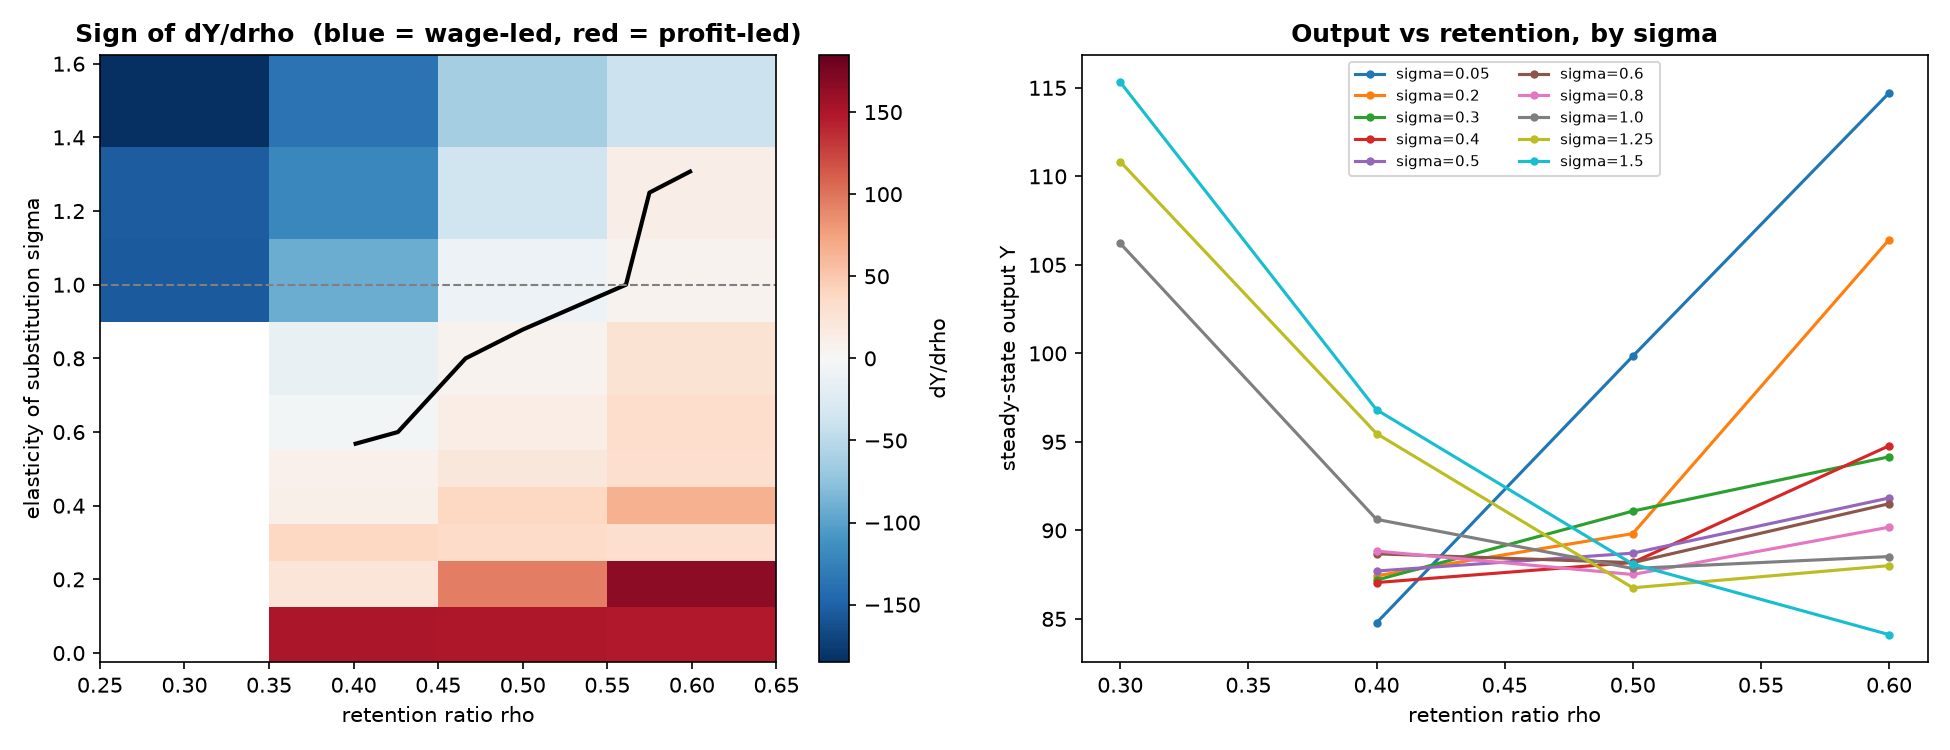
\includegraphics[width=0.82\textwidth]{ces_sign_frontier.png}
\caption{Sign of $\mathrm{d}Y/\mathrm{d}\rho$ over the $(\sigma,\rho)$ grid.}
\label{fig:frontier}
\end{figure}

\subsection{\texorpdfstring{$\sigstar$}{sigma*} is a frontier, not a number}
\label{sec:frontier-fragility}

Reporting $\sigstar = 0.654$ as a point estimate would overstate what has been
measured. Three conditioning dimensions move it materially:

\begin{itemize}
  \item \textbf{Curvature in $\rho$.} $Y(\rho)$ is significantly curved. A
  quadratic fit places the turning point \emph{inside} the support in 19 of 22
  $(c_0,\sigma)$ cells, with $|t|$ up to $20.5$. A single OLS slope fitted to a
  parabola is \emph{precise and wrong}, and this observation returns
  decisively in \cref{sec:sa}.
  \item \textbf{Choice of support.} At $c_0 = 1.0$, $\sigstar$ ranges from
  $0.46$ (on $\rho \in [0.35, 0.55]$) to $0.94$ (on $\rho \in [0.45, 0.65]$).
  \item \textbf{Choice of normalisation anchor.} Moving the anchor from
  $\rho = 0.40$ to $\rho = 0.50$ shifts $\sigstar$ from $0.84$ to $0.64$ ---
  precisely the sensitivity \citet{Temple2012} warns of, reported rather than
  suppressed.
\end{itemize}
